
\documentclass[lnicst]{svmultln}
\renewcommand{\arraystretch}{1.5}
\usepackage{amssymb}
\setcounter{tocdepth}{3}

\usepackage{epsfig}
\usepackage{cite}
\usepackage{verbatim}
\usepackage{graphicx}
\usepackage{caption}
\usepackage{subcaption}

\usepackage{url}
\urldef{\mailsa}\path|{collins, rajive}@cs.ucla.edu|
\usepackage[pdfpagelabels,hypertexnames=false,breaklinks=true,bookmarksopen=true,bookmarksopenlevel=2]{hyperref}

\begin{document}

\mainmatter  % start of an individual contribution

% first the title is needed
\title{MELON: A Persistent Message-Based Communication Paradigm for MANETs}

\titlerunning{MELON Communication Paradigm for MANETs}

\author{Justin Collins\and Rajive Bagrodia}
\authorrunning{MELON Communication Paradigm for MANETs}
% (feature abused for this document to repeat the title also on left hand pages)

% the affiliations are given next
\institute{University of California, Los Angeles\\
Los Angeles, CA\\
\mailsa }

\toctitle{MELON: A Persistent Message-Based Communication Paradigm for MANETs}
\tocauthor{Justin Collins and Rajive Bagrodia}


\maketitle
\begin{abstract}
In this paper we introduce MELON, a new communication paradigm tailored to mobile ad hoc networks based on novel interactions with a distributed shared message store. MELON provides read-only messages, per-process tracking of read messages, private messages, and bulk message operations, while addressing the dynamic and challenging environment of MANETs. After introducing the MELON, we quantitatively compare a prototype implementation to existing paradigms to show its feasibility as the basis for new MANET middleware and applications.
\end{abstract}

\section{Introduction}

While smartphones are quickly becoming ubiquitous, most networked applications continue to use a client-server model instead of communicating through mobile ad hoc networks (MANET). One reason may be the added challenges of developing a MANET application which must communicate with peers over unreliable shifting network topologies. While communicating over a single-hop wireless network (either a WiFi access point or cellular tower) to a central server is simpler, MANETs are useful when communication is between nearby devices (avoiding data charges, for example) or when there is no network infrastructure, such as in disaster recovery situations. Even less dramatic circumstances such as locations without cellular signals can also benefit from MANETs.

Applications which are developed for MANETs must operate in an infrastructureless, unreliable, and dynamic distributed environment. This presents a particular combination of challenges which should be addressed by a development platform. In \cite{mine} we identify disconnection handling, addressing and discovery, and flexible communication as important features for MANET development.

Wireless communication can be disrupted in many ways, including competing broadcasts, physical obstacles, and nodal mobility. When combined with an entirely self-organizing network where nodes may join and leave the network at any time, this environment leads to frequent communication disruptions. In traditional networking libraries, disconnections are treated as exceptional events which must be handled by the application. In MANETs, disconnections are so common they should be handled naturally by the programming paradigm.

The dynamicity of MANETs also leads to transience of resources. It is common in distributed programming paradigms to refer to resources independently from the physical location of the resources. This also works well in MANETs, since a resource is likely to be mobile, and several hosts may offer the same type of resource over time.

Before addressing resources an application must discover the resources which are available. The infrastructureless nature of MANETs precludes the use of centralized architectures to maintain a directory of resources. It is also unlikely the location of resources will be known prior to joining a network. Distributed discovery mechanisms are needed to find resources in a MANET environment.

As the primary purpose of a programming paradigm for MANETs is communication between hosts, a general-purpose paradigm should provide flexible communication: both multicast and unicast communication are common in MANET applications. Given the ubiquity of SMS, instant messaging, and direct messages, the paradigm should also support private unicast communication.

Besides the desired features for application development discussed above, it should also be noted that devices in MANETs are often resource constrained. Smartphones have become essentially ubiquitous in many countries and have much less power, CPU, memory, and storage space than a typical consumer desktop computer. These constraints may influence the design of paradigms intended to run on these limited devices.

To alleviate some of the application development challenges posed by MANETs, several approaches to middleware and libraries have been proposed. The majority of these proposals are based on traditional distributed computing paradigms: publish/subscribe\cite{psfaces}, remote procedure calls\cite{rpc}, and tuple spaces\cite{linda}. In this paper, we introduce a new paradigm for general purpose MANET applications called MELON\footnote{Message Exchange Language Over the Network} . We demonstrate that our proposed approach is feasible by comparing performance of MELON to canonical implementations of traditional paradigms.

The rest of this paper is organized as follows: Section \ref{sec:design} discusses the design and operations of MELON; Section \ref{sec:implementation} provides details of the MELON implementation; in Section \ref{sec:evaluation} we quantitatively compare MELON to existing paradigms; Section \ref{sec:relatedwork} discusses MELON in relation to existing work; and finally Section \ref{sec:conclusion} presents our conclusions.

\section{MELON Design}\label{sec:design}

The design of MELON is centered around a distributed shared message store. Each device in the network may host any number of applications which access and contribute to the shared message store. Each application hosts a local message store which may be accessed by any other local or remote application. Applications request messages (which may be stored locally or remotely) using message templates.

By communicating through a shared message store, the concept of a connection between hosts is eliminated and thus disconnections are no longer an issue at the application layer. A host suddenly leaving the network does not disrupt an application and applications do not need to handle a communication operation returning an error or failing due to intermittent network connectivity or physical wireless interference. The application is effectively insulated from these issues by the nature of the paradigm and the semantics of the operations.

Since messages are exchanged through a shared message store, messages are sent and received asynchronously with no need for a persistent connection. This provides temporal decoupling between hosts, since messages can still be delivered even after prolonged disconnections.

Due to the dynamic network topology of MANETs, maintaining any type of logical or overlay network structure becomes challenging, so MELON does not rely on a particular network structure. Discovery of available messages is performed dynamically for each operation. While this does increase the amount of communication required for each operation, it removes the need for global state and allows the network to change at any time.

MELON also provides spatial decoupling (where the sender and receiver need not be aware of each other) by matching messages based on content, rather than by a host address or location. The messages themselves may physically reside on any host in the network. The sender of a message is not aware of the receivers' identities nor even how many receivers might read a message. This frees applications from tracking remote addresses or contacting a directory service to find remote resources.

The shared wireless communication medium in MANETs is well-suited to group or multicast communications. MELON supports multicast communication by allowing any number of receivers to read the same message. MELON also provides bulk receives, which allow applications to efficiently receive multiple messages from multiple hosts in a single operation.

Applications often require point-to-point or unicast communication as well. While unicast communication can be accomplished through by storing regular messages in MELON, this communication can easily be disrupted by a process removing a message intended for a different receiver. Additionally, it is possible to eavesdrop on messages unnoticed by reading a message and not removing it. For applications such as instant messaging, it is important to have private unicast communication. In MELON, messages may be directed to a specific receiver when stored to ensure the messages are only taken by the intended recipient.

MELON also includes features uncommon to shared message stores to further simplify application development in MANETs. First, messages are returned in first-in first-out order per host. When a host receives a message request, it returns the oldest matching message in its local storage. In applications where a single host generates the majority of the messages, this eliminates the need to order messages on the receiver side. 

Secondly, MELON provides operations to only read messages which were not previously read by the same process. This enables an application to read all matching messages currently in the message store, then read only newly-added messages in subsequent operations. It also prevents an application from reading the same message twice.

Lastly, MELON differentiates between messages which are meant to persist and be read by many receivers versus messages intended to be removed from the message store. For example, messages in a news feed would have many readers, but the messages themselves should not be removed. On the other hand, a job queue expects each job to be removed by exactly one worker. MELON provides operations to support both of these scenarios.

\subsection{MELON Operations Overview}

\begin{table}
\centering
\caption{Operations Summary}
\begin{tabular}{|c|c|c|c|} \hline
& Add single message & Retrieve single message & Retrieve many messages \\ \hline
Nondestructive retrieval & \textbf{write} & \textbf{read} & \textbf{read\_all} \\ \hline
Destructive retrieval & \textbf{store} & \textbf{take} & \textbf{take\_all} \\ \hline
\end{tabular}
\label{table:opsummary}
\end{table}

Messages can be copied to the shared message store via a \textbf{store} or \textbf{write} operation. A \textbf{store} operation allows the message to later be removed from the storage space. Messages saved with a \textbf{write} operation cannot be explicitly removed from the storage space, only copied.

Messages added via \textbf{store} may be retrieved by a \textbf{take} operation using a message template which specifies the content of the message to be returned. A \textbf{take} operation will remove a message with matching content from the message store and return it to the requesting process. \textbf{take} operations are atomic: a message may only ever be returned by a single \textbf{take} operation.

A \textbf{read} operation will also return a message matching a given template, but does not remove the original message from the shared storage. Any number of processes may read the same message. However, repeated applications of a \textbf{read} operation in the same process will never return the same message. Only messages stored with \textbf{write} can be returned by a \textbf{read} operation.

The basic \textbf{take} and \textbf{read} operations return a single message per invocation. To facilitate the exchange of multiple messages, MELON includes the bulk operations \textbf{take\_all} and \textbf{read\_all}. The bulk versions operate the same as the basic operations, except all available matching messages will be returned instead of a single message. For \textbf{read\_all}, only messages which were not previously returned by a \textbf{read} or \textbf{read\_all} in the same process will be returned.

By default \textbf{take}, \textbf{take\_all}, \textbf{read}, and \textbf{read\_all} will block the process until a matching message is available. MELON also provides non-blocking versions of these operations. The non-blocking operations will return a null value if no matching messages can be found.

When a message is saved with a \textbf{store} operation, it may optionally be directed to a specific receiver. In a directed message, the identity of a receiver is included in the message as the addressee. Only the addressee may access a directed message through a \textbf{take}.

Due to the limited resources of most devices in a mobile network, storage space in MELON is explicitly bounded. Any message may be garbage collected prior to being removed by a \textbf{take} if capacity is reached.

\subsection{Operation Details}

Processes in MELON communicate by storing messages to a distributed shared message store and retrieving the messages based on templates. In this paper, we assume messages consist of an ordered list of typed values and optionally an addressee. However, nothing in the paradigm itself limits how messages might be constructed (e.g., they could be an unordered tuple with named values instead).

A message template is similar to a message, except it may contain both values and types. For example, a message containing \texttt{[1, "hello"]} could be matched by a template containing \texttt{[1, String]} or \texttt{[Integer, "hello"]} or \texttt{[Integer, String]}. A type will also match any subtypes.

Each operation is implemented as a separate function call. \textbf{store} and \textbf{write} operations have null return values and return as soon as the saved message is available in the message store. \textbf{take} and \textbf{read} operations block by default until a matching message is returned, but may be set to non-blocking on a per-call basis.

\vspace{-5 mm}
\begin{table}
\begin{tabular}{c}
\textbf{store}(\textit{message}, \textit{[address]}) $\rightarrow$ \textit{null}
\end{tabular}
\end{table}
\vspace{-5 mm}

The \textbf{store} operation takes a message as an argument and optionally an address. When called, \textbf{store} saves a copy of the message in the message store. Messages saved with \textbf{store} may only be retrieved with a \textbf{take} or \textbf{take\_all} operation. If an address is provided, then only the host with a matching identity can remove the message. Since storage space is bounded, messages may be automatically garbage collected from the storage space prior to explicit removal by a \textbf{take} or \textbf{take\_all} operation.

\vspace{-5 mm}
\begin{table}
\begin{tabular}{c}
\textbf{write}(\textit{message}) $\rightarrow$ \textit{null}
\end{tabular}
\end{table}
\vspace{-5 mm}

The \textbf{write} operation also stores a single message in the message store, but the message may only be copied from the storage space with a \textbf{read} operation, never explicitly removed. Messages written with the \textbf{write} operation may be automatically garbage collected.

\vspace{-5 mm}
\begin{table}
\begin{tabular}{c}
\textbf{take}(\textit{template}, \textit{[block = true]}) $\rightarrow$ \textit{message} or \textit{null}
\end{tabular}
\end{table}
\vspace{-5 mm}

A \textbf{take} operation requires a message template as the first argument and an optional boolean for the second argument.

The message template is matched against available messages in the message store which were added with a \textbf{store} operation. If a matching message is found, it will be removed from the message store and returned.

The block argument, which defaults to true if no argument is given, controls behavior of the operation if no matching message is available. If \textit{block} is true, the operation will wait until a matching message is available, then return it. If \textit{block} is false, the operation will return a null value.

Once a message has been returned by a \textbf{take} operation, it is removed from the message store and may not be returned by a subsequent operation in any process.

\vspace{-5 mm}
\begin{table}
\begin{tabular}{c}
\textbf{read}(\textit{template}, \textit{[block = true]}) $\rightarrow$ \textit{message} or \textit{null}
\end{tabular}
\end{table}
\vspace{-5 mm}

    The \textbf{read} operation accepts the same arguments as \textbf{take}. A \textbf{read} operation will only return messages stored with a \textbf{write} operation which have not already been read by the current process.

If a message matching the given message template is available, it will be copied and returned, but not removed from the message store. Once a message has been returned to a process, the message is considered to have been read by that process and will not be returned by any subsequent read or read\_all operations in the same process.

When a matching unread message is not available, behavior of \textbf{read} depends on the \textit{block} argument. If the argument is true or unspecified, the operation will block until a matching message is available, then return that message. If the argument is false, the operation will return a null value.

A message may be \textbf{read} by any number of processes, but only once per process.

\begin{table}
\centering
\caption{Read from multiple processes}
\begin{tabular}{|c|c|c|} \hline
\textbf{Process A} & \textbf{Process B} & \textbf{Process C} \\ \hline
\texttt{write([1, "hello"])} & \texttt{m = read([Integer, String])} & \texttt{m = read([Integer, String])} \\ \hline
\end{tabular}
\label{fig:readprocesses}
\end{table}

    Table \ref{fig:readprocesses} illustrates one process writing a single message containing the integer \texttt{1} and the string \texttt{"hello"}. Processes B and C each perform a \textbf{read} operation with the template \texttt{[Integer, String]} which matches the message stored by process A. Since \textbf{read} does not modify the storage space, the value of \textit{m} for both process B and C will be a copy of the message \texttt{[1, "hello"]} from Process A.

\begin{table}
\begin{tabular}{c}
\textbf{take\_all}(\textit{template}, \textit{[block = true]}) $\rightarrow$ \textit{array}
\end{tabular}
\end{table}

    The \textbf{take\_all} operation performs a bulk \textbf{take} on the given message template. The return value of \textbf{take\_all} is an array of matching messages. As with \textbf{take}, messages returned by a \textbf{take\_all} are removed from the shared storage and may not be returned by any subsequent operation in any process. A \textbf{take\_all} operation will not return a directed message unless the addressee matches the current process. Only messages stored by a \textbf{store} operation will be returned by \textbf{take\_all}.

    When there are no matching messages and the value of \textit{block} is \textit{true} or unspecified, the operation will block until at least one matching message is available and then return an array of available messages. If \textit{block} is \textit{false}, \textbf{take\_all} will return an empty array.

\begin{table}
\begin{tabular}{c}
\textbf{read\_all}(\textit{template}, \textit{[block = true]}) $\rightarrow$ \textit{array}
\end{tabular}
\end{table}

    \textbf{read\_all} performs a bulk read on the given message template and returns an array of matched messages. \textbf{read\_all} only returns messages which have not been previously returned in the same process by a read or \textbf{read\_all}. A \textbf{read\_all} operation will only return messages written by a \textbf{write} operation.

When there are no matching messages and the value of \textit{block} is true or unspecified, the operation will block until at least one matching message is available and return an array of available messages. If \textit{block} is false \textbf{read\_all} will return an empty array.

\begin{table}
\centering
\caption{News server and reader}
\begin{tabular}{|c|c|} \hline
\textbf{News Server} & \textbf{News Reader} \\ \hline
\begin{minipage}{2.45in}
\begin{verbatim}

function report(category, headline) {
   write([category, headline])
} 

\end{verbatim}
\end{minipage}
&
\begin{minipage}{2.5in}
\begin{verbatim}

function fetch(category) {
   return read_all([category, String])
}

\end{verbatim}
\end{minipage}
\\ \hline
\end{tabular}
\label{fig:newsreader}
\end{table}

Table \ref{fig:newsreader} demonstrates a use of \textbf{read\_all}. In this example, one or more processes generate news messages containing a news category and headline. To ensure all interested parties can read the news, the server uses \textbf{write} to disallow a reader from removing a news item and preventing other readers from reading it. Any number of processes can consume the news as readers. The \texttt{fetch} method in Table \ref{fig:readprocesses} uses \textbf{read\_all} to return all news items in a given category. Repeated calls to \texttt{fetch} will only return news items that were not already returned in a prior call.
    
\section{MELON Implementation}\label{sec:implementation}

\begin{figure}
\centering
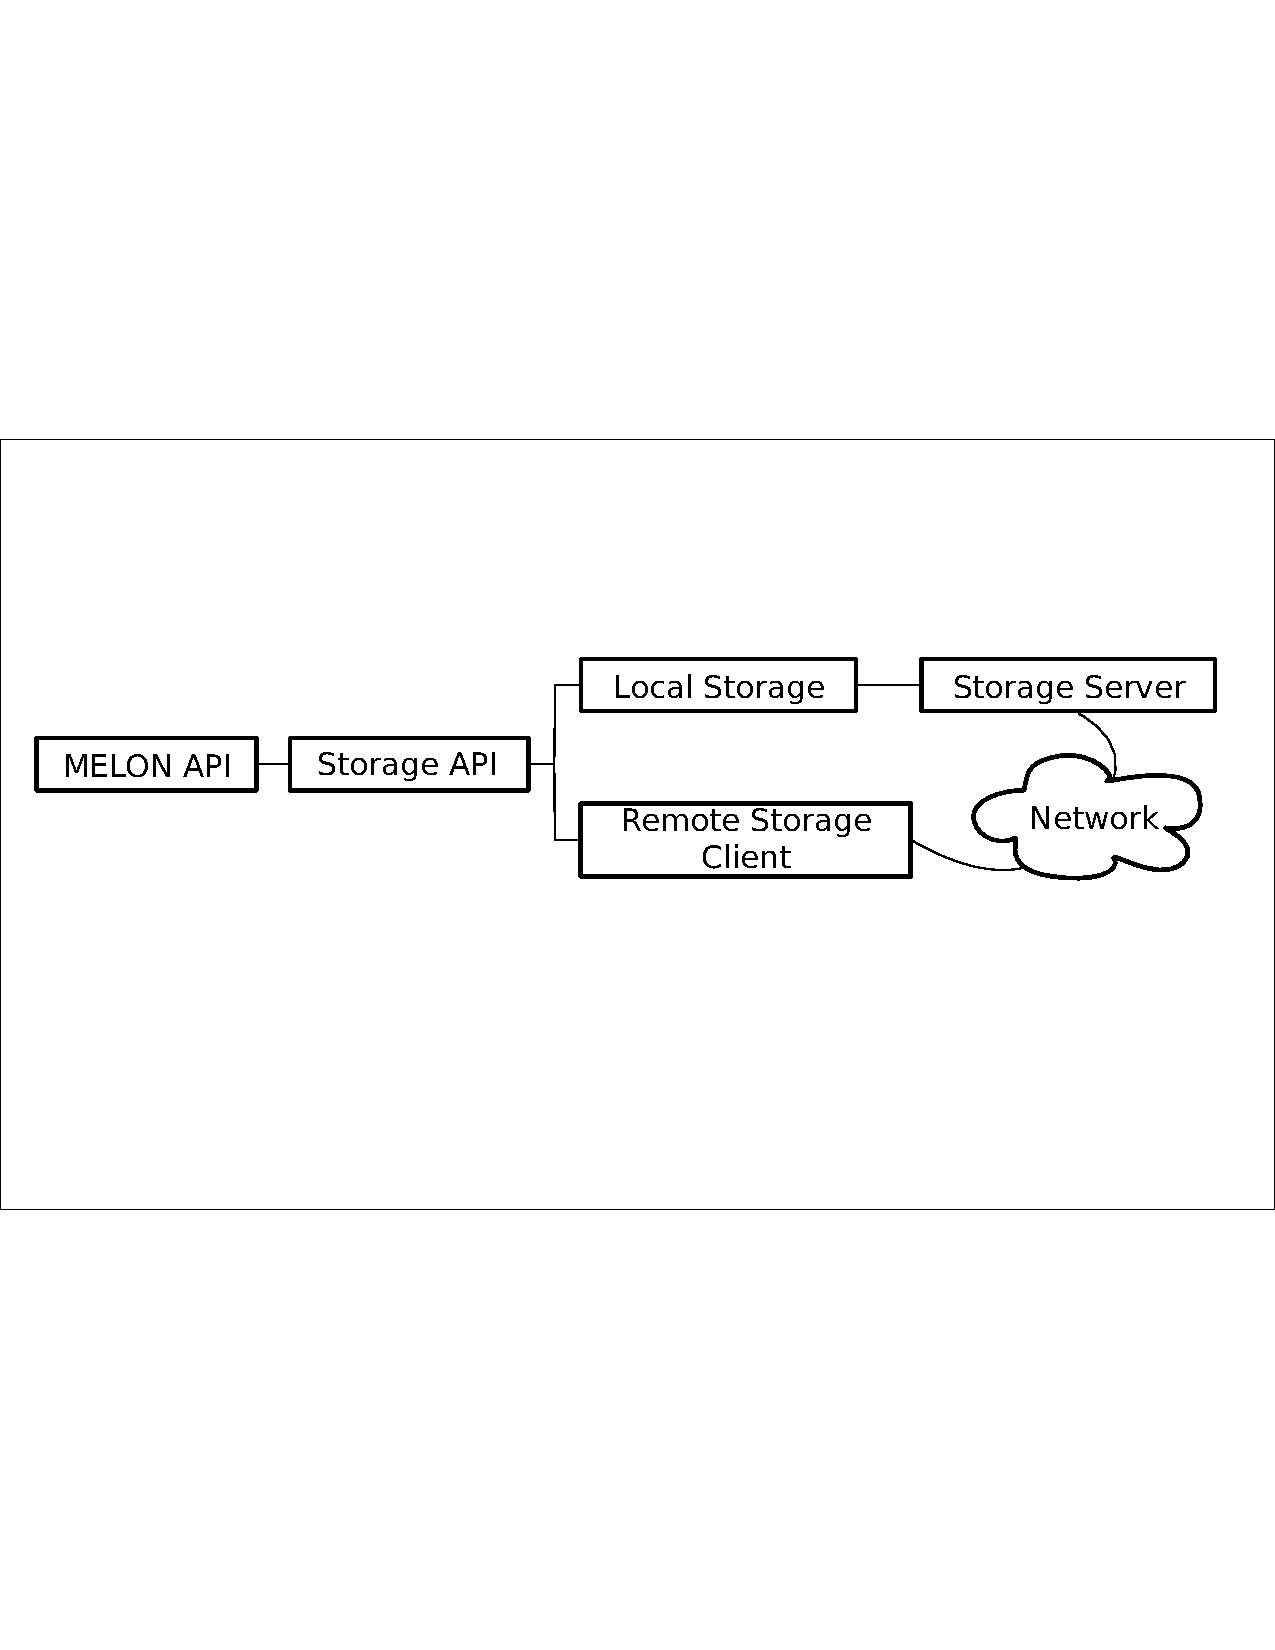
\includegraphics[scale = .30, clip, trim = 10px 280px 10px 250px]{figures/paradigm_arch.pdf}
\caption{Paradigm Architecture}
\label{fig:architecture}
\end{figure}

We developed a prototype implementation of MELON to validate our design and obtain empirical performance data. The architecture illustrated in Figure \ref{fig:architecture} is split into five parts. The MELON API is the only interface exposed to the application and provides the six operations described above. The MELON API interacts with the distributed message storage through the storage API, which provides the same interface for both local and remote storage. The storage server proves a network interface to a local storage space and accepts connections made through the remote storage stub.

Local storage is implemented simply as two dynamic arrays, one for write/read messages and the other for \textbf{store}/\textbf{take} messages. For atomic updates, the \textbf{write}/\textbf{read} array uses a readers/writer lock to allow multiple \textbf{read} operations to access the array in parallel, but locks the array for \textbf{write} operations. The \textbf{store}/\textbf{take} array does not permit concurrent operations, since both \textbf{store} and \textbf{take} modify the store. The two arrays may be accessed and modified independently.

Network communication is handled using ZeroMQ\cite{hintjens2013zeromq}, a high performance high level networking library. For the prototype, the network communication was intentionally kept simple. For example, a \textbf{read} request queries remote hosts in a random order and stops when a matching result is returned. While it is possible to improve this using multicast, it would greatly complicate the implementation by requiring the client to handle multiple asynchronous responses, choose between them, request the actual matching message, and then handle failure scenarios if the matching message cannot be returned. Our approach was to trade off potential performance gains for simplicity. 

\subsection{Tracking Read Messages}\label{sec:readmessages}

    When a messages is stored, it is given a unique identifier [\textit{P}, \textit{M}], where \textit{P} is a globally unique integer identifier for the storing process, and \textit{M} is an integer identifier for the stored message. Each process maintains an integer ID which is incremented for each store. Messages stored from the same process with sequential \textbf{store} or \textbf{write} operations will have consecutive \textit{M} values and share the same \textit{P} value.

    In order to prevent \textbf{read} from returning a message more than once in the same process, each process maintains a sparse bit set for each process from which a message has been read. The identifier [\textit{P}, \textit{M}] is condensed into a single unique integer \textit{Q} using the ``elegant pairing function''\cite{szudzikelegant} shown in Equation \ref{eq:elegantpairing}. Since the values of \textit{Q} will be consecutive integers for all consecutive values of $M < P$, it is helpful to set \textit{P} to be higher than the number of expected messages. The value \textit{Q} is then stored in a sparse bit set with a hash table using integer keys and bit field values.

 \begin{equation}
   f(M,P) = \left\{
     \begin{array}{lr}
       M^{2} + M + P & : M \geq P \\
       P^{2} + M & : M < P
     \end{array}
   \right.
   \label{eq:elegantpairing}
\end{equation}

The index \textit{i} in the sparse bit set indicates the range stored in the bit set. If \textit{w} is the number of bits for each bit set, then each bit field can store up to \textit{w} values of \textit{n}, where $w \times i \leq n < w \times (i + 1)$. A message with ID \textit{n} will be stored in index $n/w$ by setting the bit at $n \bmod w$ in the bit field to \texttt{1}.

If the index value is of size \textit{l} bits and the bit field contains \textit{w} bits, then the cost for storing a single value is $l + w$. For storing a set of consecutive values of length \textit{m}, the cost is $\lfloor \frac{m \times l}{w} \rfloor + m$ bits. In other words, the total cost is one bit per message, plus the cost of one index per \textit{w} messages.

%
%\begin{table}
%\centering
%\caption{Sparse bit set example}
%\begin{tabular}{|c|c|} \hline
%Index & Bit Field \\ \hline
%0 & 01100001 \\ \hline
%4 & 00010000 \\ \hline
%15 & 10100100 \\ \hline
%\end{tabular}
%\label{fig:bitset}
%\end{table}

Consecutive messages (from any starting value) are the best-case scenario for sparse bit sets. In the worst case, the message IDs differ by at least \textit{w}, causing each message to incur a $l + w$ cost for storage and a total cost of $m \times (l + w)$ bits.

Determining if a message [\textit{P}, \textit{M}] is in the set is accomplished by first computing \textit{Q}. If there is no key at index $Q/w$, the message has not been read. Otherwise, retrieve the bit field \textit{b} at index $M / w$. If $b \wedge 2^{M \bmod w} \neq 0$ then the message has been read, otherwise the message is unread.
    
\subsection{Retrieving Unread Messages}

When performing a \textbf{read} or \textbf{read\_all} operation, MELON must only return messages which have not previously been returned by a \textbf{read} or \textbf{read\_all} to the requesting process. Since every process has its own set of of messages which it has read, the requesting process sends this set of read messages to the requestee.

A \textbf{read} request contains a message template and the set of messages which have already been read. The receiving process will match the message template against the messages in its local storage, excluding messages which are in the set of read messages. If a matching unread message is found, the process will send the message to the requestor. If multiple matching unread messages are found, the process will send the message with the lowest message ID. If no matching messages are found, the process returns an empty response.

Similarly, \textbf{read\_all} requests also include the message template and the set of read messages. A process receiving a \textbf{read\_all} request will match the message template against messages in the local storage, excluding messages in the set of read messages. The process will then return all matching unread messages to the requestor. If no matching unread messages are found, the process returns an empty set.

\section{Quantitative Evaluation}\label{sec:evaluation}

To determine if MELON is a feasible solution for actual MANET applications, we chose to compare its performance to canonical implementations of publish/subscribe, RPC, and tuple spaces. If a prototype implementation of MELON performs at least as well as existing paradigms, then it is likely to be useful in actual practice. In the experiments below, we compare speed of operations, message overhead, throughput, and latency in a MANET context.

\subsection{Experimental Setup}

In order to judge the performance of MELON, we used applications written using the prototype MELON implementation and evaluated them using the EXata network emulator\cite{exata}. Using an emulator allowed us to run real applications but also have precisely repeatable environments and scenarios with high fidelity network models.

Two scenarios were used for our experiments. In the first, 11 nodes are placed in static positions which force routes to be at least two hops. In the second, 50 nodes move using random waypoint at approximately walking speeds (maximum of 10m/s), signal propagation is limited to 50m in order to match an indoor environment, and the two-ray model is used for path loss. Every run of the mobile scenario uses the same random seed so the mobility pattern is identical. In both scenarios, 802.11b WiFi is used with the DSR\cite{dsr} routing protocol.

The experiment coordination application described in the next section was used to run the applications and gather results in a consistent manner.

\subsubsection{Experiment Coordination Application}

\begin{figure}
\centering
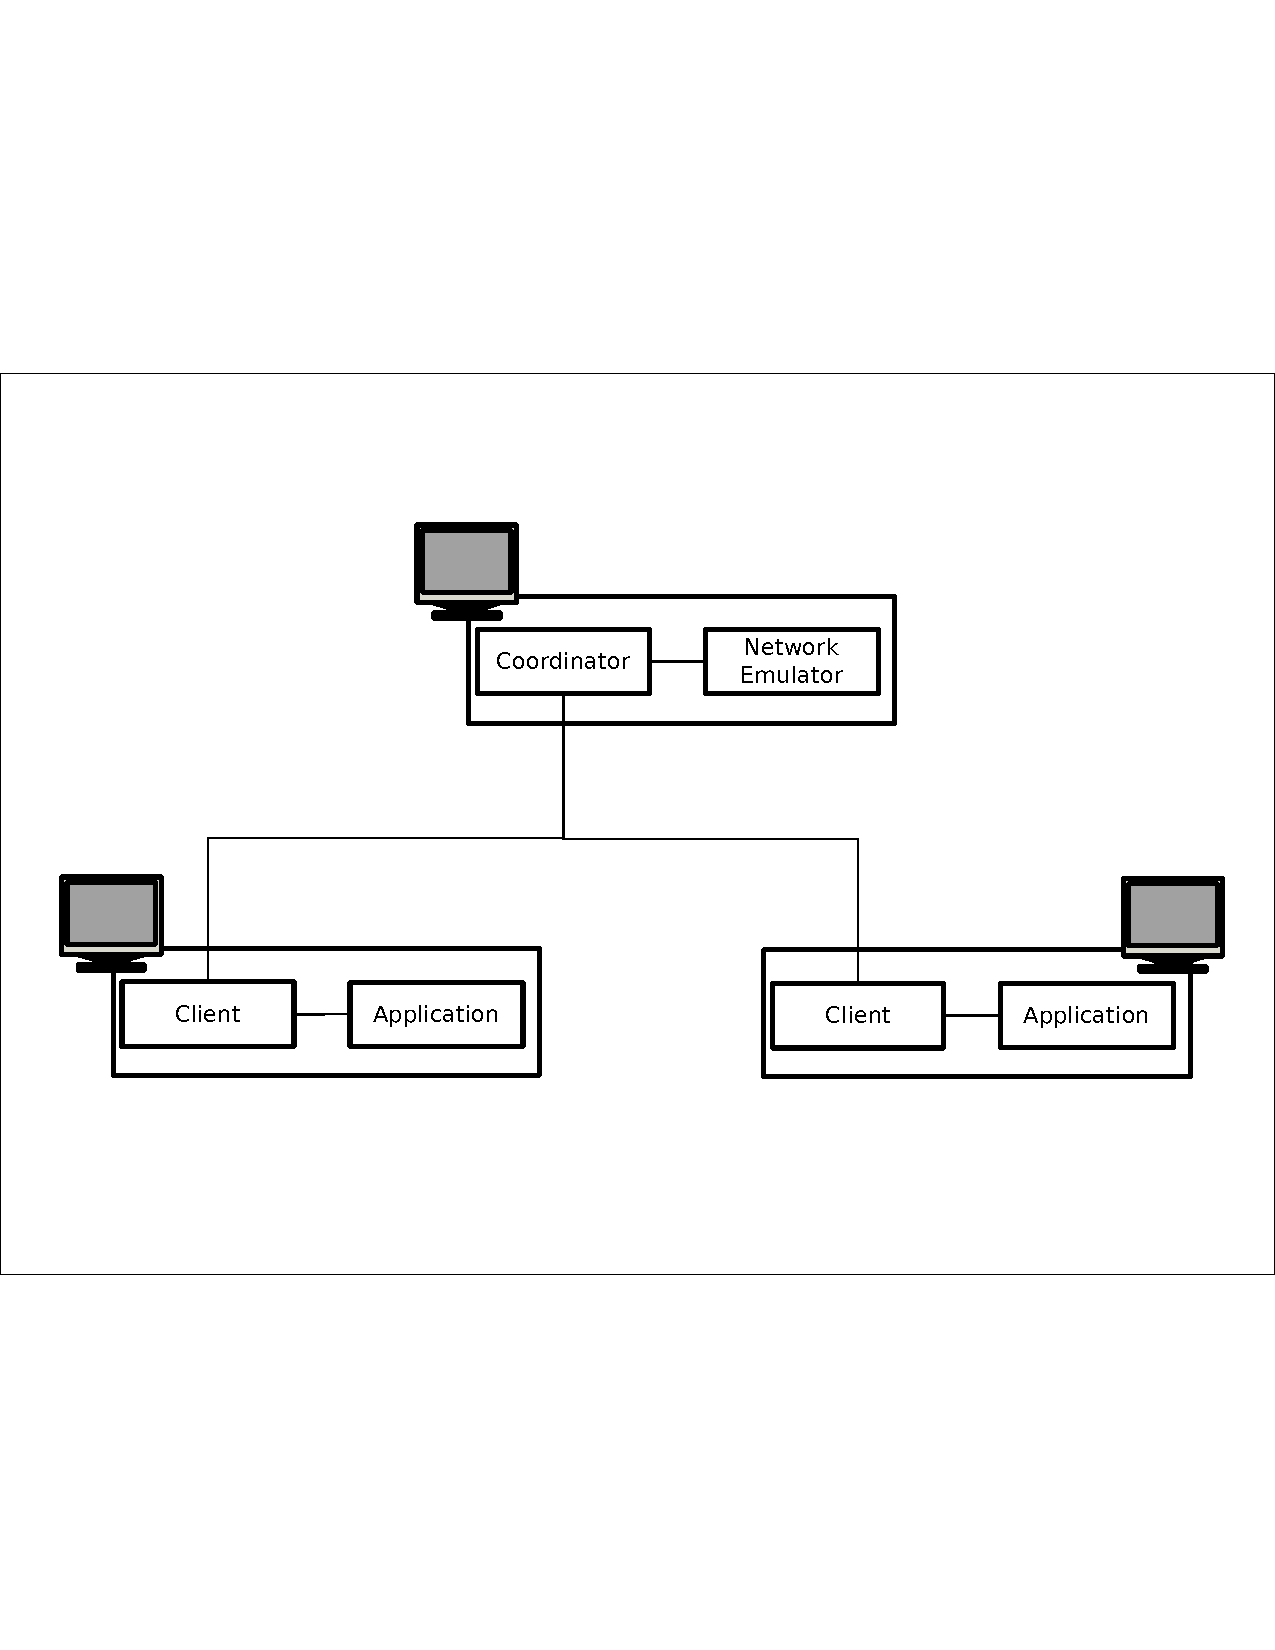
\includegraphics[scale = .34, clip, trim = 94px 279px 24px 252px]{figures/experiment_arch.pdf}
\caption{Coordinator Architecture}
\label{fig:coordarchitecture}
\end{figure}

To ease the process of repeatedly setting up experiments, we developed an experiment coordination framework written with MELON. The application handles running real applications on multiple hosts, executing the network emulator, and gathering results into a single location.

The architecture of the framework is illustrated in Figure \ref{fig:coordarchitecture}. For simplicity, the coordinator resides on the same host as the network emulator. The coordinator sends out commands to clients which reside on each host. The clients are responsible for executing programs on their local host and sending resulting output to the central coordinator.

The coordinator first writes a job containing the command to execute and any relevant options. Each client reads the job, starts the command, then stores a confirmation once the application is initialized and ready to begin. When the coordinator has taken a confirmation from each host, it starts the network emulator, then writes a ``go'' message. Upon reading the go message, each client signals the application to begin.

As the application runs, the client gathers output and stores it. When the application finishes, it signals that it is done and then awaits a kill signal from the client. The client also stores a ``done'' signal. When the coordinator has taken a ``done'' message from each client, it collects the results and then sends a ``stop'' message. The clients then stop the applications and the framework is ready to start the next experiment.

\subsection{Operation Speed}

\begin{figure}
\centering

\begin{subfigure}{.5\textwidth}
\centering
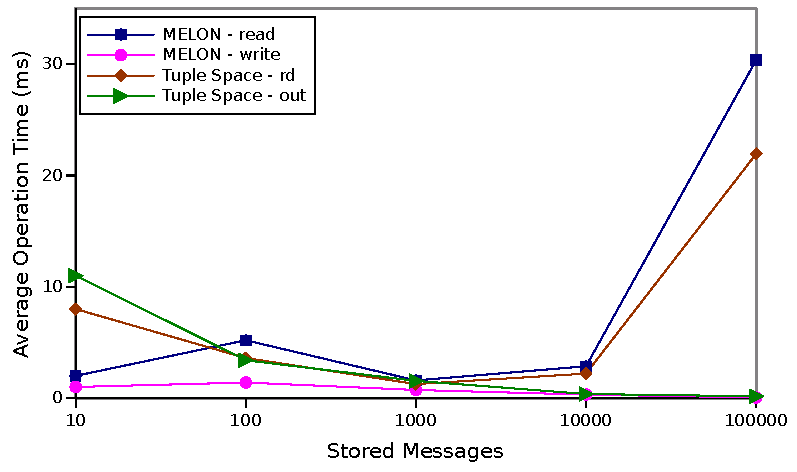
\includegraphics[width = \linewidth, clip, trim = 0px 0px 0px 0px]{figures/read_speed.pdf}
\caption{Read Speed}
\label{fig:readspeed}
\end{subfigure}%
\begin{subfigure}{.5\textwidth}
\centering
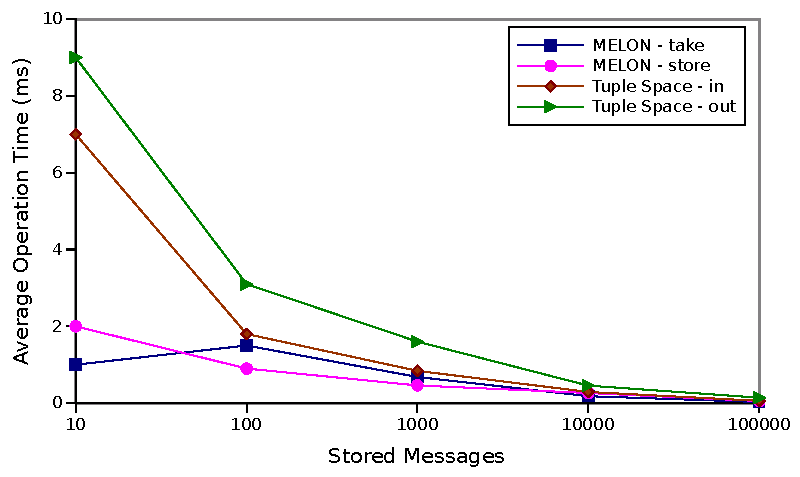
\includegraphics[width = \linewidth, clip, trim = 0px 0px 0px 0px]{figures/in_speed.pdf}
\caption{Take Speed}
\label{fig:takespeed}
\end{subfigure}

\caption{Operation Speeds}
\end{figure}

To establish a baseline for performance, we measured the time for the \textbf{write}, \textbf{read}, \textbf{store}, and \textbf{take} operations directly on a local message storage and compared the results to the LighTS\cite{lights} local tuple space implementation used by LIME. In these experiments, all messages are first stored, then either read or removed from the local storage. No network communication is involved.

When comparing \textbf{read} and \textbf{rd}, we simulate the MELON's feature of only returning unread messages by using a sequential integer ID in the tuples and performing a \textbf{rd} operation for each ID. If we did not do this, LighTS would return the same tuple for each \textbf{rd} operation.

In both LighTS and MELON, messages are stored in what is essentially an array. Since we are not removing messages, each operation must linearly search the array taking O(\textit{nm}) time, where \textit{n} is the length of the message or tuple and \textit{m} is the number of stored messages or tuples. Naturally, operations returning messages near the beginning of the array are faster, while the slowest operation returns the last message in the array. In our experiments, this cost did not become apparent until searching 100,000 messages. The average time per operation from 10,000 to 100,000 increased \~9x for LighTS and \~10x for MELON, with total read time taking just under a minute. It is unsurprising MELON is slightly slower, since it must also check that a message is not in the ``read'' list before returning it.

On the other hand, removing messages is naturally quite fast, since the matching message is always the first message in the store. All \textbf{take}/\textbf{in} operations require less than 8\textit{ms} to execute on average. MELON is slightly faster here due to differences in how removal is implemented, although average speed per operation converges as the number of operations performed increases.

Storing messages is faster than removing them for both implementations. In LighTS there is slightly more constant overhead for adding new tuples, so \textbf{out} operations are a little slower than \textbf{write} and \textbf{store} in MELON.  However, in reality both implementations are plenty fast for typical applications, since storing a message takes less than 10\textit{ms} on average, and usually less than 4\textit{ms}.

Overall, MELON performs roughly the same or better than LighTS when performing serial operations.

\subsection{Communication Overhead}

\begin{figure}
\centering
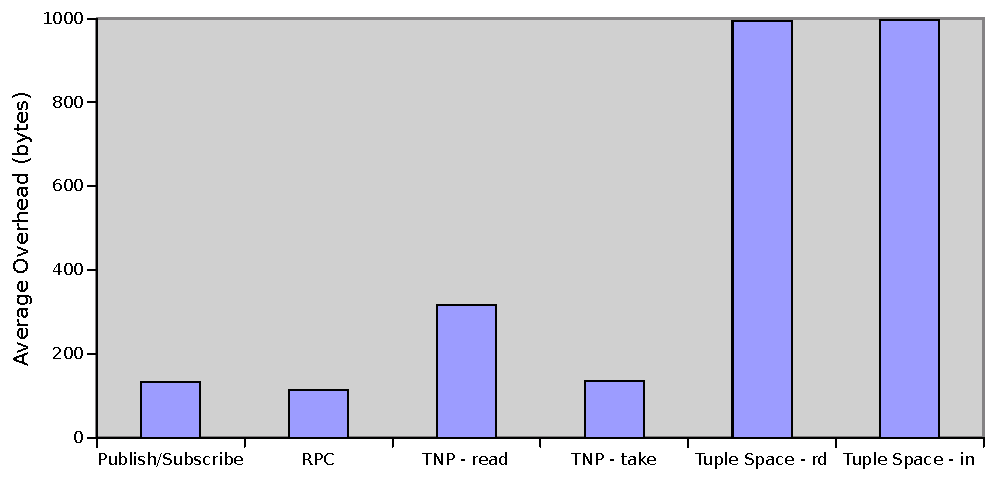
\includegraphics[scale = .50, clip, trim = 0px 0px 0px 0px]{figures/overhead.pdf}
\caption{Message Overhead}
\label{fig:overhead}
\end{figure}

For any communication library or framework, the message size added by use of the library is an important factor in determining its usefulness. In these experiments, we measure the number of bytes actually sent over the network, divide by the number of messages sent (in this case, 1000) and subtract the 1KB application payload. This leaves us with the overhead introduced by the paradigm. We compare the overhead of MELON to canonical implementations of publish/subscribe, RPC, and tuple spaces in Figure \ref{fig:overhead}.

Publish/subscribe and RPC have very low overhead and provide a good baseline. In the case of publish/subscribe, the only added information to a publication is the topic. Periodic subscription messages are small and infrequent compared to the number of messages sent. For RPC, there is one initial exchange to find the remote object, then later messages only need the object and method names plus the payload itself.

As in the operation speed experiments, we use the LighTS tuple space implementation. The serialized versions of tuples and tuple templates are very large and must be sent for each request. If a simpler data structure were used, overhead would be expected to be similar to MELON's overhead for \textbf{take}.

For MELON, \textbf{take} and \textbf{read} requests must send a message template, so the size of the request is dependent on how many values the template contains. For \textbf{read} operations, each request must also send information on previously read messages as described in Section \ref{sec:readmessages}, which increases as the number of read messages increases.

\subsection{Message Latency}

\begin{figure}
\centering

\begin{subfigure}{.5\textwidth}
\centering
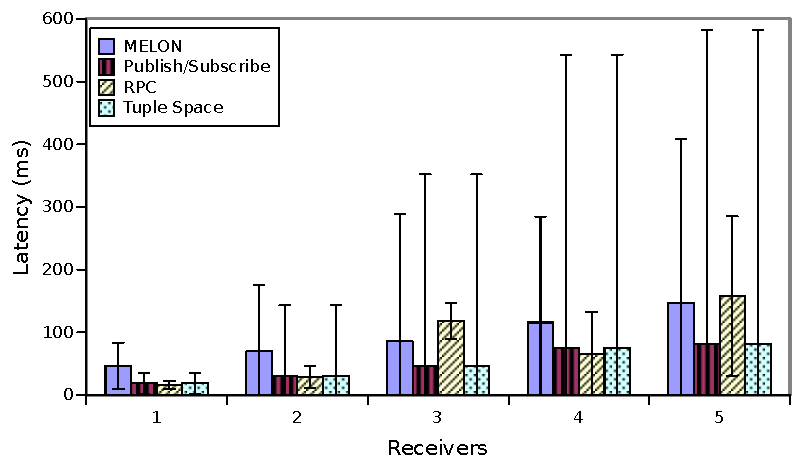
\includegraphics[width = \linewidth, clip, trim = 0px 0px 0px 0px]{figures/latency_static.pdf}
\caption{Static Scenario}
\label{fig:latencystatic}
\end{subfigure}%
\begin{subfigure}{.5\textwidth}
\centering
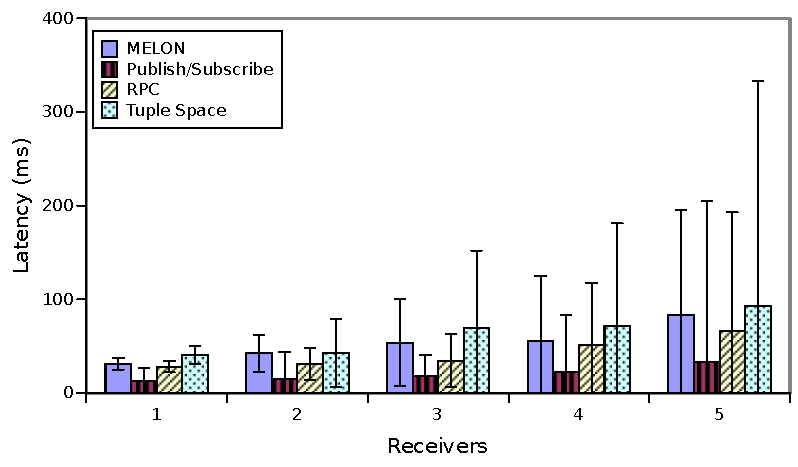
\includegraphics[width = \linewidth, clip, trim = 0px 0px 0px 0px]{figures/latency_mobile.pdf}
\caption{Mobile Scenario}
\label{fig:latencymobile}
\end{subfigure}

\caption{Message Latency}
\end{figure}

Figures \ref{fig:latencystatic} and \ref{fig:latencymobile} show the average latency between a client's request for a message and the receipt of a matching message. The error lines indicate the standard deviation. In these experiments, a single host writes out 1,000 messages with a 1KB payload, and the other hosts concurrently read the messages. Tuple spaces and MELON used the \textbf{rd}/\textbf{read} operations to retrieve the messages one at a time, rather than the bulk retrieval with \textbf{rdg} or \textbf{read\_all}. Since publish/subscribe does not involve a ``request'' beyond the initial operation, latency was measured as the time elapsed between receiving sequentially numbered publications.

MELON does show higher average latency rates in the static scenario, although for three or more receivers the standard deviation is lower than the other paradigms. In the more realistic mobile scenario, however, MELON latency is about the same or slightly lower than tuple spaces. Comparing the static and mobile scenarios also demonstrates one of the issues in wireless networks: the mobile scenario allows distinct routes to form between hosts with less interference, while the static scenario has many collisions causing more communication delays even though the distance between devices is smaller.

\subsection{Message Throughput}

\begin{figure}
\centering

\begin{subfigure}{.5\textwidth}
\centering
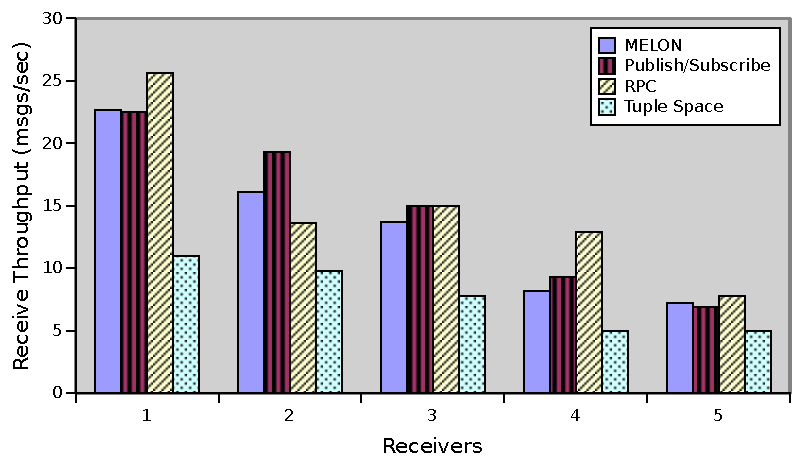
\includegraphics[width = \linewidth, clip, trim = 0px 0px 0px 0px]{figures/throughput_static.pdf}
\caption{Static Scenario}
\label{fig:throughputstatic}
\end{subfigure}%
\begin{subfigure}{.5\textwidth}
\centering
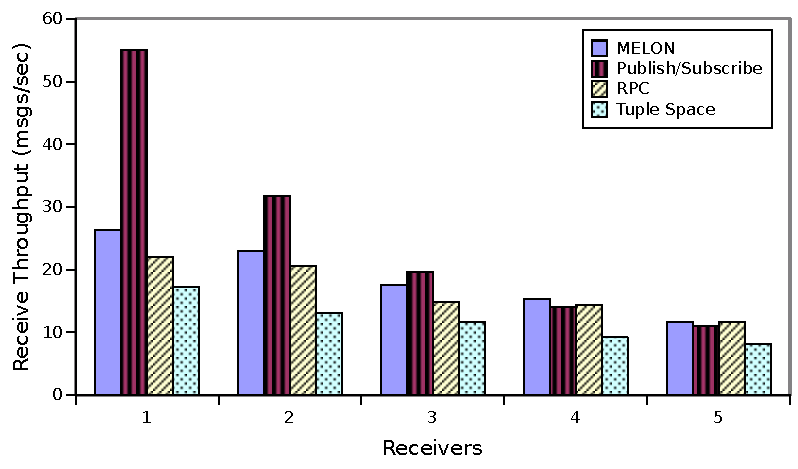
\includegraphics[width = \linewidth, clip, trim = 0px 0px 0px 0px]{figures/throughput_mobile.pdf}
\caption{Mobile Scenario}
\label{fig:throughputmobile}
\end{subfigure}
\caption{Message Throughput}
\end{figure}

Throughput in these experiments was measured on the receiver side in terms of messages delivered per second. As in the other experiments, 1,000 messages with a 1kb payload are output by one host, while the other hosts read the messages one at a time. Figures \ref{fig:throughputstatic} and \ref{fig:throughputmobile} show the average throughput as the number of receivers increases.

Publish/subscribe dominates in these experiments since it is the only push-based paradigm, allowing the sender to publish messages at a high rate without requests or acknowledgments from the receivers. Also, subscribers may receive multiple publications concurrently which increases throughput capacity.

Despite having higher average latency than the other paradigms, MELON demonstrates good throughput in both the static and mobile scenarios. However, throughput for all paradigms drops off dramatically as more receivers are added. Also, all paradigms performed better in the mobile scenario than in the static scenario. This is likely due to two factors: devices were not forced to be more than one hop apart, and the large number of devices allows distinct routes between devices and decreases wireless broadcast collisions.

\section{Related Work}\label{sec:relatedwork}

The concept of a distributed shared message store is based on the idea of tuple spaces introduced with the Linda\cite{linda} coordination language. Several projects have adapted tuple spaces to MANETs, including LIME\cite{lime}, MESHmdl\cite{meshmdl}, TOTA\cite{tota}, and EgoSpaces\cite{egospaces}, of which LIME is likely the most well-cited example.

The original version of LIME relies on explicit join and leave operations to federate distributed tuple spaces, which is at odds with the frequently unexpected disconnections in MANETs. \cite{limerevisted} discusses the difficulties LIME encounters when attempting to implement tuple space semantics, including situations that can lead to livelocks. LIME II\cite{lime2}, Limone\cite{limone}, and CoreLIME\cite{corelime} are projects intended to address the shortcomings in the original LIME.

REDS\cite{reds} and GREEN\cite{green} are examples of publish/subscribe adapted to MANETS. AmbientTalk\cite{ambienttalk} is an entire language for MANETs based on RPC and actors. Further surveys of middleware, languages, and communication paradigms for MANET development can be found in \cite{mine} and \cite{mwtrends}.

\subsection{Comparison to Existing Paradigms}

This section compares MELON to publish/subscribe, remote procedure calls (RPC), and tuple spaces: three distributed computing paradigms often used as the basis for MANET middleware.

\subsubsection{Disconnection Handling}

In the unreliable MANET environment, disconnections frequently occur during the exchange of messages. Since disconnections can be prolonged, the networking layers will assume the connection is entirely lost and cease retrying. By having a message persist in some way, a paradigm can overcome these disconnections and deliver the message at a later time.

Publish/subscribe allows message publication without any consideration for the state of the subscribers. Publish/subscribe itself does not specify how ``missed'' publications should be handled. A publish/subscribe system can utilize ``brokers'' which manage subscriptions and facilitate delivery of publications. Brokers can then serve as message buffers and provide more reliable message delivery in the face of disconnections. In distributed publish/subscribe systems, however, the brokers must be self-organizing, and in MANET this is complicated by how quickly the network can change. It is common for distributed publish/subscribe systems not to provide message persistence. If a subscriber is not available at the time of publication, the message will not be received.

Since RPC requires a connection for communication, disconnections typically cause RPC to block a process entirely until a remote node hosting an appropriate method is available. Messages themselves only exist briefly during the RPC transaction. Messages cannot be sent if a connection cannot be made to a remote host.
    
In tuple spaces and MELON, message persistence is inherent in the paradigms. In both paradigms, exchange of messages is achieved by storing the messages in a shared storage space. Any amount of time may elapse between the storage of a message and its retrieval. This allows reliable communication even in the face of prolonged disconnections and is the reason we have chosen it for MELON.

\subsubsection{Addressing and Discovery}

All of the paradigms discussed here provide indirect addressing of resources separated from the physical machines. Publish/subscribe uses topics or content to deliver message to subscribers, RPC uses class and method names, and tuple spaces and MELON retrieve messages by matching content to templates. While all three traditional paradigms originally relied on centralized services (brokers from publish/subscribe, service directories for RPC, and a centralized database for tuple spaces), simple distributed versions may be implemented by having each node act as part of a distributed service.
    
\subsubsection{Flexible Communication}

A general purpose communication paradigm for MANET applications should have the flexibility to support both unicast and multicast communication.

Publications in publish/subscribe are inherently multicast, since any number of nodes can subscribe. Unicast communication is much less comfortable in publish/subscribe, as it involves negotiating which topics should be used to identify which nodes. Publish/subscribe also does not provide any mechanism for ensuring or even acknowledging message delivery to any given subscriber, especially since publishers and subscribers are intended to be unaware of each other.

Since RPC mimics local method calls, it is natural that RPC is best suited for unicast communication, in which the message is the argument to the method and the return value is the response from the remote host. Assuming multicast RPC functions in the same manner, then a multicast RPC invocation would expect multiple return values, one from each remote host. In a MANET, it is likely not every remote host would reliably return a response, further complicating the semantics. A typical RPC invocation would block waiting for a response, but it is not practical to wait for all responses to a multicast RPC invocation when some responses may never be received. The use of futures or asynchronous callbacks can improve the situation, but causes semantics to differ even more from unicast RPC.

Tuple spaces are naturally multicast, since any number of nodes may read a given tuple. Unicast communication can be achieved by using a field in the tuple as the recipient’s address. The recipient then performs in operations on tuples with their address in order to receive the tuples.

MELON divides communications into three types: messages which can be received by any single recipient, messages which can be received by a specific single recipient, and messages which can be received by any number of recipients. Messages sent with a store operation can only be consumed by a single take operation. Directed messages are also sent with store, but can only be consumed with a take performed by the intended recipient. write stores messages which may be read by any number of recipients and can never be removed by a take. MELON also provides the ability to receive multiple messages at once with \textbf{take\_all} and \textbf{read\_all} operations.
    
Networked applications also commonly require private, unicast communication. For example: SMS services, direct messaging in social networks, or communication of sensitive data. For our purposes, private communication is the exchange of messages between two parties which cannot be disrupted or eavesdropped upon by a third party from within the context of the paradigm itself. In other words, concerns such as encrypting data or sniffing network traffic would be outside the paradigm context.

RPC is unicast by default and there is no method in the paradigm for eavesdropping or disrupting RPC between two nodes. However, RPC has a different complication: remote hosts are generally identified by their exposed methods and there is no mechanism for attaching identity to the hosts. RPC will connect to any remote method with the expected API. So while private communication is the default in RPC, there is an addressing issue which makes it complicated to communicate with a specific recipient.

Communication in publish/subscribe is public and multicast by nature. Any subscriber can subscribe to any set of publications, making it simple to eavesdrop on communications. Bidirectional communication is also difficult in publish/subscribe, since there is no information attached to a publication indicating the identity of the publisher. This is by design, but it complicates situations in which two hosts need to dialog.

In tuple spaces, tuples are public and available to any recipient. Not only can any node read any communications without detection, any node can also disrupt communications by removing tuples intended for a specific recipient.

MELON provides two access control mechanisms for messages. First, messages are explicitly either available for any recipient to remove or limited to read-only operations. Read-only messages are useful in scenarios where information is intended to be widely available and removal of the information would be considered disruptive to the application. Second, if messages are directed to a specific recipient, then the paradigm implementation is responsible for disallowing any other nodes from reading or removing the given message. This allows simple private unicast communication between nodes.

\subsubsection{Multiple Read Problem}

The multiple read problem \cite{mrdp} is specific to tuple spaces: in a situation where the tuple space contains many tuples of interest, how do multiple readers read \textit{all} relevant tuples? In tuple spaces, the non-destructive \textbf{rd} operation returns a copy of a matching tuple, but it may return the same tuple any number of times since the tuple is chosen nondeterministically between all matching tuples. In many tuple space implementations, this occurs because the tuples are stored sequentially and so the first matching tuple is always the same\cite{de2012new}.

One solution is to use a single tuple as a mutex, lock the tuple space, remove all matching tuples with \textbf{in}, then replace them in the tuple space. However, this ruins any concurrency the tuple space could have had with multiple readers.

Another solution is to provide a bulk \textbf{rd} operation to return all matching tuples. However, once a ``snapshot'' of the tuple space has been taken with a bulk \textbf{rd}, new matching tuples may be introduced. A second bulk \textbf{rd} would return both the old (already seen) tuples and the new tuples. A similar suggestion from \cite{edwards2001jini} is to remove all matching tuples inside a transaction, then abort the transaction in order to actually leave the tuple space unmodified. However, this again leaves the problem of separating new tuples from previously-read tuples.

MELON avoids this issue by only returning messages unread by the current process. Assuming a fixed set of stored messages, repeated \textbf{read} operations in the same process would eventually return each matching message exactly once. MELON also provides the \textbf{read\_all} operation for reading messages in bulk. Unlike the tuple space version, \textbf{read\_all} only returns unread messages. This allows applications to easily read all existing matching messages, after which \textbf{read\_all} will only return messages stored since or unavailable during the previous operation.

\section{Conclusion}\label{sec:conclusion}

MELON is a new communication paradigm designed for MANET application and middleware development. It provides a unique combination of new features for interacting with a distributed shared message store, including separation between read-only messages and removable messages, private messages, bulk message operations, and tracking of read messages. In this paper we used real applications to compare MELON performance to existing communication paradigms and demonstrated the new paradigm has acceptable overhead and performance in a MANET context, as well as being useful for general purpose applications.

There are several aspects of MELON which can be explored in future work including message replication, garbage collection, and secure communication. Message replication is very useful in MANETs to overcome network partitioning and increase availability. On the other side, garbage collection of old (and replicated) messages is necessary to keep the MELON storage requirements low for small devices. While MELON does offer direct communication, actually encrypting private communications is necessary for true security against eavesdropping.

\bibliographystyle{unsrt}
\bibliography{refs}

\end{document}
